\documentclass{article}
\usepackage{graphicx}
\usepackage{amsmath}
\usepackage{hyperref}
\usepackage{amsmath}
\usepackage{amsfonts}
\usepackage{parskip}
\usepackage{cleveref}
\usepackage{xcolor} 
\setlength{\parindent}{0em}
\usepackage[margin=1.0in]{geometry}
\begin{document}

\begin{flushleft}
    \textbf{\large{Problem Set \#4}} \\
    MACSS 3000, Prof. Evans \\
    Benjamin Rothschild
\end{flushleft}

\section*{Problem 1}
\subsection*{Part A}
\begin{center}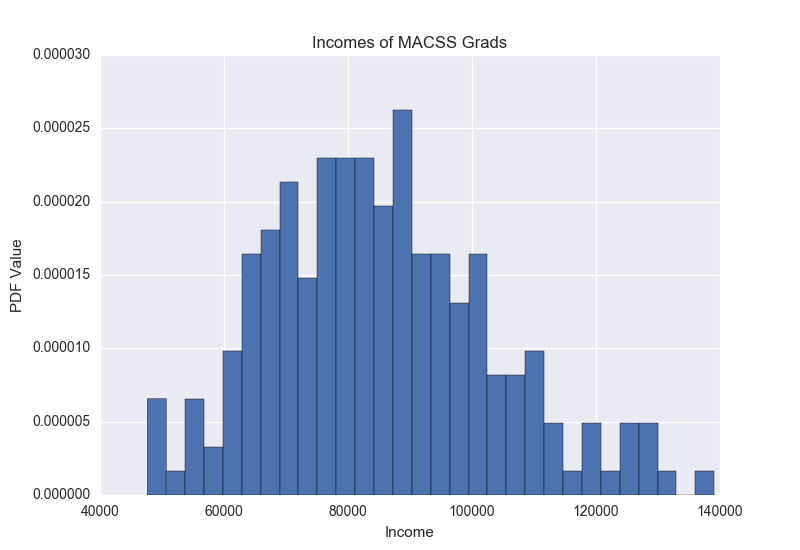
\includegraphics[width=100mm]{images/1a.png}\end{center}

\subsection*{Part B}
The result of my \texttt{LN\_pdf(np.array([[200.0, 270.0], [180.0, 195.5]]))} is
\begin{center}
  \begin{tabular}{ c | c }
    \hline
    0.0019079 & 0.00123533 \\ \hline
    0.00217547 & 0.0019646 \\
    \hline
  \end{tabular}
\end{center}

\subsection*{Part C}
Criterion value is: 9.82687615e-14 at $\mu$ = 11.33 and $\sigma$ = 0.21.
\begin{center}
  \begin{tabular}{ l | c | c }
    \hline
     & model & data \\ \hline
    $\mu$ & 85276.81 & 85276.82 \\ \hline
    $\sigma$ & 17992.54 & 17992.54 \\ \hline
    \hline
  \end{tabular}
\end{center}
\begin{center}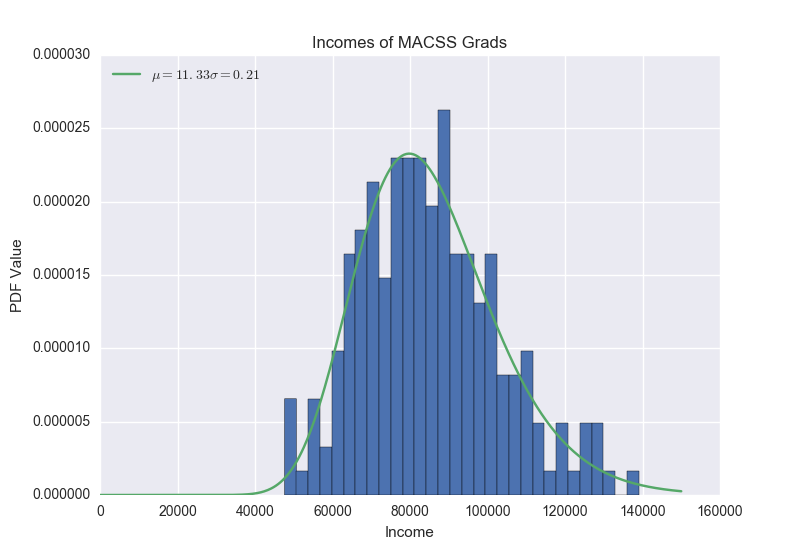
\includegraphics[width=100mm]{images/1c.png}\end{center}


\subsection*{Part D}
Criterion value is: 0.04772766 at $\mu$ = 11.32 and $\sigma$ = 0.21.
\begin{center}
  \begin{tabular}{ l | c | c }
    \hline
     & model & data \\ \hline
    $\mu$ & 84949.77 & 85276.82 \\ \hline
    $\sigma$ & 18009.17 & 17992.54 \\ \hline
    \hline
  \end{tabular}
\end{center}
\begin{center}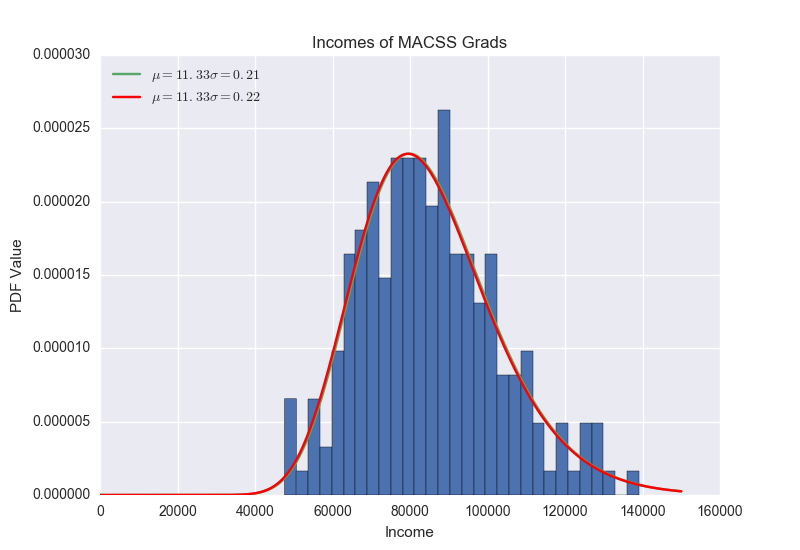
\includegraphics[width=100mm]{images/1d.png}\end{center}
The results from the two SMM methods are very similar.

\end{document}